\documentclass[letterpaper,twocolumn,amsmath,amssymb,pre]{revtex4-1}
\usepackage{graphicx}% Include figure files
\usepackage{color}

\newcommand{\red}[1]{{\bf \color{red} #1}}
\newcommand{\blue}[1]{{\bf \color{blue} #1}}
\newcommand{\green}[1]{{\bf \color{green} #1}}

\newcommand{\fixme}[1]{\red{[#1]}}
\newcommand{\davidsays}[1]{{\color{red} [\green{David:} \emph{#1}]}}
\newcommand{\renesays}[1]{{\color{red} [\blue{Rene:} \emph{#1}]}}
\newcommand{\jeffsays}[1]{{\color{red} [\blue{Jeff:} \emph{#1}]}}

\newcommand\micron{\ensuremath{\mu\text{m}}}

\begin{document}
\title{Robustness of MinD oscillation in \emph{Escherichia coli} with
  diverse cell shapes}

\author{Jeff B. Schulte}
\affiliation{Department of Physics, Oregon State University}
\author{Rene W. Zeto}
\affiliation{Department of Physics, Oregon State University}
\author{David Roundy}
\affiliation{Department of Physics, Oregon State University}

\begin{abstract}
  The dynamics of the Min-protein system help Escherichia coli
  bacteria regulate the process of cell division by identifying the
  center of the cell.  We model the Min-protein system in bacteria
  that have been forced into unusual flattened shapes, as have
  recently been experimentally observed.  We find that although the
  presence of Min oscillations is robust in a wide variety of cellular
  configurations, the location of the peaks is strongly affected by
  the cellular shape.  In some cases no periodic oscillations are
  observed.  In particular, we find that cellular shapes observed
  experimentally to present irregular oscillations do so in the
  theoretical model, consistently \fixme{or inconsistently?} with
  experiment.  \fixme{In agreement with previous theoretical and
    experimental results, we observe ``rotating'' behavior in certain
    shapes having three corners.}
\end{abstract}

\maketitle

\section{Introduction}
\fixme{Huang and those who reference him use the terms 'numerical
  deterministic reaction-diffusion model' and 'stochastic version of
  this model' for the stochastic.} It is vital that during the process
of bacterial cell division a cell avoid minicelling, or splitting into
daughter cells with lopsided volumes.  Instrumental to this process in
\emph{Escherichia coli} is a long FtsZ polymer chain that develops on
the cell wall in the center region of the cell, helping dictate the
plane of
division~\cite{adams2009bacterial,lutkenhaus2007assembly}. Previous
experimental studies have shown that the MinC protein, known to
inhibit the FtZ polymer\cite{shen2010examination}, exhibits pole to
pole oscillatory behavior between both ends of the wild-type
pill-shaped cell.  It thus has a higher time averaged concentration in
the cell poles than in the center region, which aides in prohibiting
the FtZ from developing in the wrong region.  The MinC is recruited to
these poles by MinD, which ineracts with another protein, MinE, that
is neccesary for MinD oscillation.~\cite{hu1999topological,
  fu2001mine, shapiro2009and, yu1999ftsz, raskin1999rapid}.

Previous studies have shown that the minD protein system is capable of
exhibiting oscillations in round shapes as well as in connected three
pronged tube shapes~\cite{varma2008min}, in which the oscillations
seem to seek out the extreme poles in the
cell~\cite{corbin2002exploring} \cite{juarez2010changes}. However,
Mannik \emph{et al.} have also shown that there are limitations to
this capability~\cite{mannik2010bacteria}
\cite{mannik2009bacterial}. They have experimentally forced E. Coli
cells into flattened irregular shapes of $0.25\mu m$
thickness. Oscillations in this type of cell shape lose their
regularity, both temporally and spatially. This allows for an
opportunity to test previously studied MinD simulation models against
more extreme experimental cases than have been seen thus far.

A significant amount of work has been done to develop protein reaction
and diffusion models that exhibit accurate macroscopic dynamics of the
MinD protein system. Early models involve free proteins that affect
each others' rates of diffusion and membrane attachment, but do not
combine into compound states~\cite{meinhardt2001pattern}.  In 2003
Huang improved upon this work with a simple and very successful
simulation model based on MinD-MinE combination, ATPase hydrolysis,
and MinD membrane attachment that exhibits accurate MinD oscillations
in cylindrical cells~\cite{huang2003dynamic}. In this model
cytoplasmic MinD is more likely to attach to the membrane when MinD is
already clustered there (following observed non-linear attachement of
minD on the cell membrane), and is stationary once attached.  A number
of studies have used an approach similar in that they do not rely on
the ability of MinD to move along the walls and
cluster~\cite{kruse2007experimentalist, meinhardt2001pattern,
  drew2005polymerization, fange2006noise, kerr2006division}, while
studies have been made as well of models which rely on MinD mobility
and attraction on the cell membrane~\cite{kruse2002dynamic,
  howard2005cellular}.  Experimental studies of the Min system's
association with the cell membrane have also been
made~\cite{hsieh2010direct,mileykovskaya2003effects}.

Variations of the Huang 2003 model that stochasticly account for
variations of molecular
interaction~\cite{kerr2006division,fange2006noise} and monte-carlo
simulations that implement this stochastic version of Huang's mean
field reaction rates confirm the major results obtained by Huang's
model, and more successfully predict experimentally observed
oscillations in round cell phenotypes~\cite{fange2006noise,
  huang2004min}. The successful simulations of three pronged cells
mentioned above are stochastic
simulations~\cite{varma2008min}. Biochemical models of broader scope
have also been used to study the MinD system and show consistent
results~\cite{arjunan2010new}.

\fixme{There are not any direct comparisons of the deterministic and
  stochastic methods that I can find other than the fange2006 paper
  cited above for the round cells.  Those showed that the
  deterministic couldn't predict oscillations in perfectly round
  cells, but could in almost round ellipses.  It seems that once the
  stochastic methods began to be used, nobody really used the
  deterministic method any longer.  Not sure what to say about this in
  order to introduce what we do here properly.}

In this paper we apply a deterministic method and a stochastic method
of simulation and compare them against Mannik's experimental findings.


\fixme{Following paragraph is awkward, and I don't think it's needed.}
Studies have shown as well that MinD binds preferentially to regions
enriched with cadiolipin, an anionic phospholipid that collects on
regions of high negative curvature. This mechanism has been
incorporated into other
models.\cite{drew2005polymerization,cytrynbaum2007multistranded,renner2012mind,renner2012mind}
However, this mechanism of combined clustering, phospholipids and MinD
has not been observed in real cells. \cite{halatek2012highly}


\begin{figure}
  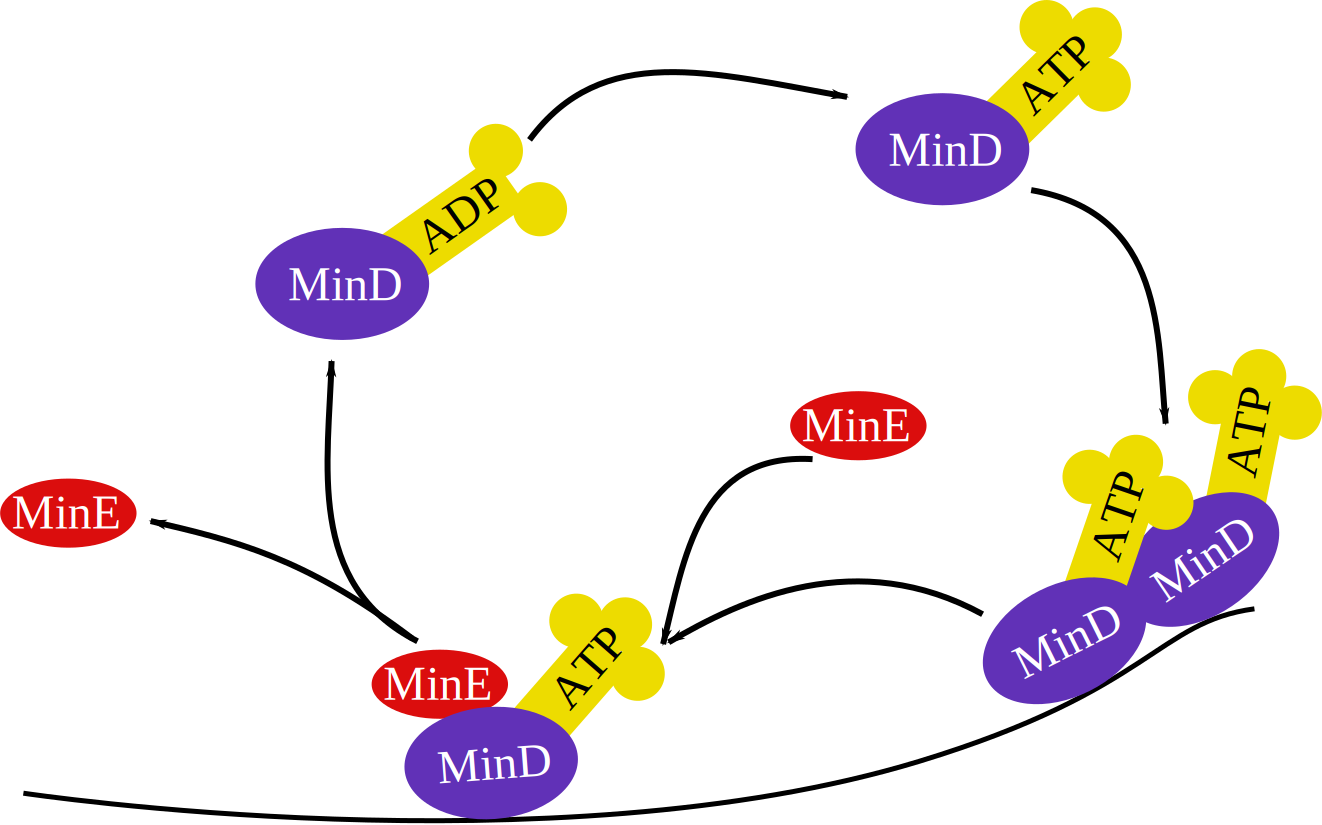
\includegraphics[width=\columnwidth]{reactions}
  \caption{Reactions included in the model of Huang \emph{et
      al.}~\cite{huang2003dynamic}.}\label{fig:reactions}
\end{figure}


\section{Model, Methods, and Cell Shapes}\label{sec:model-method-shapes}
We implement the reaction-diffusion model of Huang \emph{et
  al.}~\cite{huang2003dynamic}.  Figure~\ref{fig:reactions} shows the
reaction process.  The cytoplasmic MinD:ADP complex undergoes
nucleotide exchange and is changed into the MinD:ATP complex.  This
will naturally diffuse and attach to the cell membrane.  A cytoplasmic
MinE will attach to the wall bound MinD:ATP complex and after a time
will activate ATP hydrolosis.  This breaks up the complex, releasing
MinE, phosphate, and MinD:ADP back into the cytoplasm.  The MinD:ADP
will undergo nucleotide exchange and begin again the cyclic process.
The model is defined by a set of five reaction-diffusion equations:

\begin{multline}
  \frac{\partial \rho_{D:ADP}}{\partial t} = \mathcal{D}_D\nabla^2\rho_{D:ADP}-k_D^{ADP\rightarrow ATP}\rho_{D:ADP}\\
  +\delta(d_w)k_{de}\sigma_{DE},\hspace{3.4cm}
\end{multline}
\begin{multline}
  \frac{\partial \rho_{D:ATP}}{\partial t} = \mathcal{D}_D\nabla^2\rho_{D:ATP}+k_D^{ADP\rightarrow ATP}\rho_{D:ADP}\\
  -\delta(d_w)[k_D+k_{dD}(\sigma_D+\sigma_{DE})]\rho_{D:ATP}
\end{multline}
\begin{multline}
  \frac{\partial \rho_E}{\partial t} = \mathcal{D}_E\nabla^2\rho_E+\delta(d_w)k_{de}\sigma_{DE}
  -\delta(d_w)k_E \sigma_D \rho_E
\end{multline}
\begin{multline}
  \frac{\partial \sigma_D}{\partial t} = -k_E\sigma_D\rho_E
  +[k_D+k_{dD}(\sigma_D+\sigma_{DE})]\rho_{D:ATP}
  \label{eq:d-on-wall}
\end{multline}
\begin{multline}
  \frac{\partial \sigma_{DE}}{\partial t} = -k_{de}\sigma_{DE}+k_E\sigma_D\rho_E\hspace{3cm}
  \label{eq:FifthPDE}
\end{multline}

where $\rho$ is cytoplasmic protein density ($\mu m^{-3}$), $\sigma$
is membrane bound density ($\mu m^{-2}$), $\mathcal{D}_D$ and
$\mathcal{D}_{E}$ th diffusions constants for MinD and MinE,
respectively, $k_D^{\textrm{ADP $\rightarrow$ ATP}}$ the rate of
conversion from MinD:ADP to the MinD:ATP complex, $k_D$ the rate of
MinD:ATP attachement to the membrane when no protein is already
attached there, $k_{dD}$ the increase of this rate when MinD:ATP is
present on the membrane, $k_{de}$ the rate of hydrolisis of the
MinD:MinE:ATP complex, $k_E$ the rate of cytoplasmic MinE binding to
membrane bound MinD:ATP complex, and $d_w$ is the distance from the
point in space to the closest wall (which will always be
perpendicular to this distance).  $\delta(d_w)$ has units of
$\mu m^{-1}$ and will be zero everywhere except at the wall.
Equations \ref{eq:d-on-wall} and \ref{eq:FifthPDE} will only be
relevent at the membrane because the membrane bound density values
will have no meaning in the cytoplasm where there is no membrane.

Our diffusion and reaction rates are shown below.  We are interested
primarily in the effect of cellular size and shape on the protein
oscillations, so we follow Huang\cite{huang2003dynamic} and do not
deviate from the wild type values used in the cited work (see values
below).  Huang's simulations use total MinD and MinE concentrations of
$1,000/\mu m$ and $350/\mu m$, respectively, in a cylindrical cell of
radius $0.5\mu m$, and in our (non-cylindrical) cells we use the same
number of proteins per unit volume.  These concentration values are
1273 $\mu m^{-3}$ and 446 $\mu m^{-3}$, respectively. \fixme{It's been
  a while so might want to check this to make sure it's true.}
\begin{gather*}
  \mathcal{D}_D = \mathcal{D}_{E} = 2.5\micron^2/\text{sec}\\
  k_D^{\textrm{ADP $\rightarrow$ ATP}} = 1/\textrm{sec,  }
  k_D = 0.025 \micron /\textrm{sec}\\
  k_{dD} = 0.0015 \micron^3/ \textrm{sec,  }
  k_{de} = 0.7/\textrm{sec}\\
  k_E = 0.093 \micron^3 /\textrm{sec}.
\end{gather*}
A 3D grid is then constructed in cartesian coordinates, with a grid
spacing of .05\micron.

We have performed both a basic finite analysis, deterministic
simulation that is spatially and temporally discrete, and a stochastic
analysis that is spatially discrete but continuous in time.  Our
stochastic simulation method follows the work of
Kraus~\cite{kraus1996crosstalk} which in turn follows a method
introduced by Gillespie~\cite{gillespie1977exact}.

\begin{figure*}
  %\includegraphics[width=\textwidth]{../data/shape-p/3_00-0_50-0_00-0_00-15_00-exact/plots/image-plot}
  \includegraphics[width=\textwidth]{../data/shape-p/3_00-0_50-0_00-0_00-15_00-exact/plots/single-image-plot}
  \includegraphics[width=\textwidth]{../data/shape-p/3_00-0_50-0_00-0_00-15_00-full_array/plots/single-image-plot}
  \caption{Contour plot images of the concentration of each protein
    species in a natural pill-shaped bacterium at regular intervals in
    time (one second intervals), with darker regions indicating higher
    concentration. The upper plots shows results from the
    deterministic simulation and the lower shows results from the
    stochastic simulation.  The cells pictured are $4\micron$ in
    length, measured from end to end.  The order of frames is such
    that individual MinD proteins begin at the bottom of the plot (in
    the MinD:ATP state in the cytoplasm), and progress upward until
    they reach the MinE:MinD:ATP membrane-bound complex.  At that
    point, they will spontaneously dissociate into cytoplasmic MinE
    (the top row) and the starting state of cytoplasmic MinD:ADP.  The
    densities plotted are integrated along the axis orthogonal to the
    page, and the color scale is chosen separately for each species
    with black as the maximum value over space and time.  The
    stochastic densities are smeared out over space using a guassians
    approximation developed by Zhang et all~\cite{zhang2007gaussian}}.
  \label{image-p}
\end{figure*}

We mean to investigate the geometric limits of the Min system
oscillations as observed by Mannik \emph{et
  al.}~\cite{mannik2012robustness}, so we model the Min system in a
variety of cell shapes and sizes.  Here we present a selection of
these, first naturally occuring pill-shaped cells and then a number of
flattened out shapes which reflect the experiments of Mannik \emph{et
  al.}, in which bacteria are confined within a thin slit of height
$0.25\micron$ ~\cite{mannik2012robustness}. Viewed from the top down
the cells will show the shapes described below and viewed from the
side they show at their edges a semicircular protrusion (one may
imagine the shape of a pancake). We have simulated and analyzed a
number of these flattened shapes in addition to those shown below,
including equilateral and iscosolese triangle shapes, shapes shaped
like greater than signs, '$>$', and four-pronged 'starfish' shapes.
For all of these we have varied the cell size, expanding the two
dimensions that are tangent to the flattened surface from very small,
'steady state' scales (which we discuss below) to scales twice that of
the published Mannik shapes.  Our conclusions are based on all of this
data, but we present here specific, illustrative examples: two
flattened shapes that are designed to replicate those published by
Mannik and two `stadium' shapes that respectively have the same
quadrupole moments of the two Mannik shapes.

%% Our pill shapes differ from those of Huang \emph{et al.} in that they
%% are cylinders with hemisphere endcaps instead of pure cylindrical
%% shapes.  Our cylinderidrical radius is $0.5\micron$ and the lengths
%% of our cells (measured between the tips of the endcaps) are
%% $5\micron$, $4\micron$, $3\micron$, and $2.5\micron$.

\fixme{Is the following Kubitscheck paragraph needed?}
Kubitschek has shown in multiple experiments that at the time of cell
division cells have a volume that is within a range of roughly
$1\micron^3$ to $2\micron^3$~\cite{kubitschek1990cell,
  kubitschek1968linear}.  We follow Huang's
simulations\cite{huang2003dynamic} and Mannik's experiments and model
cells that are slightly larger than this range.

\begin{figure*}
  %\includegraphics[width=\textwidth]{../data/shape-p/3_00-0_50-0_00-0_00-15_00-exact/plots/image-plot}
  \includegraphics[width=\textwidth]{../data/shape-p/3_00-0_50-0_00-0_00-15_00-exact/plots/single-image-plot}
  \includegraphics[width=\textwidth]{../data/shape-p/3_00-0_50-0_00-0_00-15_00-full_array/plots/single-image-plot}
  \caption{Contour plot images of the concentration of each protein
    species in a natural pill-shaped bacterium at regular intervals in
    time (one second intervals), with darker regions indicating higher
    concentration. The upper plots shows results from the
    deterministic simulation and the lower shows results from the
    stochastic simulation.  The cells pictured are $4\micron$ in
    length, measured from end to end.  The order of frames is such
    that individual MinD proteins begin at the bottom of the plot (in
    the MinD:ATP state in the cytoplasm), and progress upward until
    they reach the MinE:MinD:ATP membrane-bound complex.  At that
    point, they will spontaneously dissociate into cytoplasmic MinE
    (the top row) and the starting state of cytoplasmic MinD:ADP.  The
    densities plotted are integrated along the axis orthogonal to the
    page, and the color scale is chosen separately for each species
    with black as the maximum value over space and time.  The
    stochastic densities are smeared out over space using a guassians
    approximation developed by Zhang et all~\cite{zhang2007gaussian}}.
  \label{image-p}
\end{figure*}

Huang \emph{et al} ~\cite{huang2003dynamic} has has performed a linear
stability analysis on the model which shows an upper limit on a steady
state solution of $2\mu m$.  Cells with dimensions longer than this
are unstable and show oscillatory behavoir in this direction, where
cells that are shorter relax into a motionless steady state.  We have
similarly performed a stability analysis in an infinite slab with a
thickness equal to our flattened cells ($0.25\mu m$) and have found
that an equivalent stability limit for half wavelengths is $2.13\mu
m$. As expected, when decreasing the lengths and widths of our
simulated flattened cells so that the shortest distance across the
cell is less than this length, the cells stop exhibiting any
oscillalitory behavior.  The deterministic simulations relax into a
motionless state and the stochastic simulations exhibit multiple
random locations of small maximization.

\section{Naturally Occuring Pill Shaped Cells}

We begin with the naturally occuring pill cell shape.  We peice this
shape together as two hemispherical endcaps attached on either end of
a cylinder.  This shape follows the early simulations of Huang
\emph{et al.} but differs in that we have added the end caps for a
more natural shape, expecting similar results.

This simple cell shape is a good starting point for observing in
detail the dynamic interaction between the different stages of protein
that lead to their qualitatively distinct behavoir. Figure
\ref{image-p} shows the process in a series of frames taken from
simulation animations for both the deterministic and stochastic
simulations.  We have 'smeared out' the stochastic concentrations in a
manner meant to reproduce the images shown by diffraction limited
flourescence microscopy.  We do so using the two dimensional gaussian
approximation developed by Zhang et all~\cite{zhang2007gaussian}.  In
this approximation we use a numerical aperture value of 1.3, which is
the same as used by mannik experimentally, and a wavelength of
$650nm$.  Each frame is 2.5 seconds ahead of the last, and each image
shows the concentration of a given state of protein (of the five
described in the reaction model) summed over the coordinate orthogonal
to the page.  The color scale for each protein state is set according
to the maximum values observed.

Figure~\ref{image-p} begins about 300 seconds into the simulation and
shows a typical period of oscillation that in the pill shape repeates
itself with a high degree of regularity, for both the deterministic
and stochastic simulations.  At $t=0$ the cytoplasmic MinE is
concentrated in the upper portion of the cell and is diffusing
downward, where it will react with and stick to wall-bound MinD that
is concentrated on the membrane in the lower portion of the cell.
This process is in fact already well on its way, as seen by the
significant concentration of wall bound MinD:MinE which is creeping
down to the lower corner, removing the MinD from the membrane as it
goes.  The removed MinD (cytoplasmic MinD:ADP) diffuses freely for a
time before spontenously undergowing nucleotide exchange and shifting
back into the MinD:ATP that is able to attach to the membrane.
Diffusing a small distance away from the bottom of the cell will bring
the protein into the MinE collection, where reactions will prevent it
from collecting for any significant time on the membrane.  Diffusing
further towards the upper end, however, while the MinE has not yet
collected there, will allow MinD:ATP to accumulate with the other
MinD:ATP, which is seen at seconds 10 through 15 in
Figure~\ref{image-p}.  Eventually the MinE creeps all the way down to
the bottom of the cell where it slowly runs out of wall bound MinD to
react with, before diffusing back up and starting again on the upper
portion of the cell. This is seen in seconds 15 through 20 in the
figure.  \fixme{There is another paragraph after this in the latex
  that I commented out because I thought we might be spending too much
  time on the description}

%%  At 15 seconds, the membrane-bound MinD:ATP has
%% been essentially removed from the top end of the cell, and MinD:ATP
%% has begun to bind to the membrane in the the lower half of the cell.
%% At this stage, there is a high concentration of cytoplasmic MinE at
%% the top of the cell, and by 16 seconds we begin to see the formation
%% of a MinE ring just below the center of the cell.  At 18 seconds, the
%% cell has reached its original state (reversed directionally), with
%% MinD:ATP bound to the membrane on the lower third of the cell, a high
%% concentration of cytoplasmic MinE in the upper half of the cell, and a
%% MinE ring pushing downward on the membrane-bound MinD:ATP.

We test cells of radius $.5\micron$ and of lengths $2\micron$,
$3\micron$, $4\micron$, and $5\micron$ measured from the tip of one
end cap to the tip of the other \fixme{I'm running the 2,3,5 pills
  again to make sure that everything in this paragraph is true}. In
each case, we observe in the deterministic simulations a quick
establishement (within a few periods) of regular oscillatory behavoir
that lasts indefinitely.  This temporal regularity can be seen in
Figure~\ref{corr-pill}, which shows the temporal correlation of the
total MinD protein located in the the two polar sections of the cell.
In the stochastic simulations the pills exhibit coherence times of
over 7 periods and the determinisitic version cohere indefinately.

\begin{figure}
  \includegraphics[width=\columnwidth]{../data/shape-p/3_00-0_50-0_00-0_00-15_00-full_array/plots/correlation-rl.pdf}
  \caption{No caption}
  \label{corr-pill}
\end{figure}

While the stochastic results show periods that seem to have a high
degree of regularity as well as similarity to the deterministic
results, they do differ in the precise locations of the maxima.  While
the deterministic simulations show maxima that are every time
concentrated in the center of one of the cell ends, with a symmetric
smear of protein going out laterally to either side, the stochastic
simulations show maxima that, while always located somehwere in the
polar region of the cell, occur at different positions within this
region.  This is reflected in Figure~\ref{image-p}, which shows
periods that are the same and qualitative behavoir that is
approximately the same, but also that there is variation in the
details of the stochastic simulation maxima location.


\fixme{Is the table of the cell periods needed? I'm not sure if we
  have a experiment to compare this to} The stochastic results show
oscillitions that are similarly regular in time, with periods that
nearly match those of the deterministic (they differ roughly by a
factor of .05) \fixme{does this square with the correlation data
  periods?}. The regularity of the pill shape cell periods is
discussed below, in our analysis of time correlation data \fixme{not
  written yet}.  These periods increase with cell length, as shown in
Table~\ref{tab:pill-periods}, in agreement with the results of Huang
\emph{et al.}.


\begin{table}
  \begin{tabular}{|r|c|c|c|l|}
    \hline Length($\mu$) & 2.50 & 3.00 & 4.00 & 5.00\\ \hline
    Period(sec) & sim & 33 & 38 & 48 \\ \cline{2-2} \hline
  \end{tabular}
  \caption{Period of oscillation according to length of cell for
    pill-shaped cells.}\label{tab:pill-periods}
\end{table}

\begin{figure*}
  \centering
  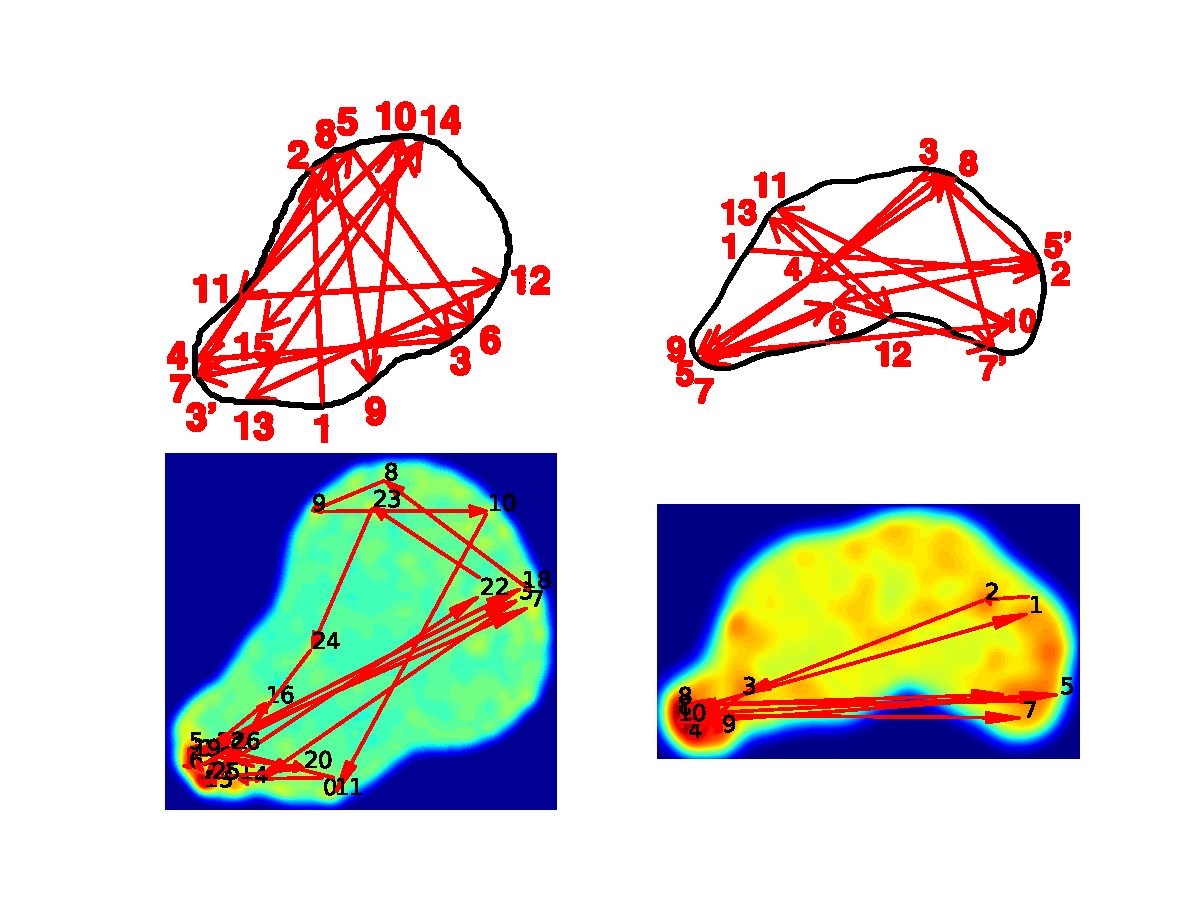
\includegraphics[width=\textwidth]{../paper/plot-ave}
  \caption{We display here arrows depicting successive maxima in space
    and and time overlayed on a color plot of the total MinD density
    averaged over the same time period.  The simulation time covered
    for the flattened cells is \fixme{340} seconds, which is the same
    period of time depicted in the experimental data plots of Mannik
    \emph{et al.}~\cite{mannik2012robustness}.  For the wild type pill
    shape, we only cover \fixme{???} seconds, in order to provide a
    useful comparison due to its shorter oscillation period.  The top
    row shows plots published by Mannik of the MinD maxima behavoir
    and the bottom two rows show our simulations using the stochastic
    and deterministic algorithms, respectively.  We simulated
    approximations to the two shapes observed by Mannik, which we call
    \emph{shape A} and \emph{shape B}.  In addition, we studied two
    flattened stadium shapes which we call \emph{stadium A} and
    \emph{stadium B} corresponding in aspect ratio and thickness to
    the two experimental shapes.  The spatial length scale of all the
    figures shown was identical. Each of the flattened cell shapes
    uses the same color scale for the number of proteins per unit
    area.  Finally, we display the natural pill shape, which was also
    featured in Figs.~\ref{image-p} and~\ref{corr-pill}, with a
    different color scale to reflect the thicker cell containing more
    proteins per cross-sectional area.  }
  \label{randst-plot-ave}
\end{figure*}

\section{Comparison of Mannik's Experimental and Our Stadium Shapes}

As describe in Section~\ref{sec:model-method-shapes}, we will focus on
simulation of four flattened cell shapes: two shapes copied from
Mannik's experiment~\cite{mannik2012robustness} (shape~\emph{A} and
shape~\emph{B}), and for comparison two symmetrical stadium shapes
that have the identical aspect ratio, thickness and volume (stadium
\emph{A} and stadium \emph{B}).  These stadium shapes enable us to
distinguish between the effect of cellular irregularity and that of
overall size and aspect ratio.  We note that shape \emph{B} is more
irregular than shape \emph{A}, and in particular features a prominant
region of concavity on its left-hand side.  For each of these shapes
(in addition to the wild type pill shape discussed previously) we have
simulated in excess of \fixme{???} seconds of evolution of the MinD
system using both the deterministic model of Huang~\fixme{cite} and
the stochastic model of Huang~\fixme{cite}.

From each of these flattened simulations, we have chosen a typical 350
second segment to compare with the results of Mannik exemplified in
arrow plots in which the arrow heads show the location of sequential
MinD maxima within the cell (over the same time
interval)~\cite{mannik2012robustness}.  This comparison is shown in
Fig.~\ref{randst-plot-ave}.  In addition to arrows between successive
maxima in space and time, we plot as a colored background the density
of MinD protiens averaged over the same time period.  We note that we
have manually verified that our (computer-generated) arrow plots also
reflect a human interpretation of a movie of the same data.  Finally,
for comparison we present the same plot for a wild-type cell, with a
time period of \fixme{???}  seconds to account for its short period of
oscillation.  In every case, including the wild type pill shape, we
see irregularity in the location of the maxima when using the
stochastic approach.  The deterministic method shows uniformly bipolar
oscillation, with the exception of shape \emph{B}, which develops weak
intermediate maxima on the right-hand edge of the cell.

%% We found that the deterministic simulations of the MinD system results
%% in robust and regular oscillatory behavoir of polar selection and
%% oscillation in not only symmetrical shapes, such as the wildtype pill
%% shape, but also in very assymetrical, flatttened cells, such as those
%% observed by Mannik.  We also examined larger and smaller versions of
%% these shapes, and found this behavior to be very robust, from the
%% minimum size to sustain oscillation (around \fixme{???} $\mu$m) up to
%% around twice the cell size reported by Mannik.  At larger sizes than
%% this, less regular oscillations occur using the deterministic method,
%% but we note that the cells reported by Mannik are already considerably
%% larger in volume than typical wild type
%% cells~\cite{kubitschek1990cell,kubitschek1968linear,mannik2012robustness}.

\begin{figure}
  \includegraphics[width=\columnwidth]{../data/shape-randst/0_25-18_50-18_50-95_00-15_00-full_array/plots/correlation-rl.pdf}
  \includegraphics[width=\columnwidth]{../data/shape-stad/0_25-2_35-1_32-0_00-15_00-full_array/plots/correlation-rl.pdf}
  \caption{Correlation for A shapes}
  \label{fig:corr-pancake-A}
\end{figure}

The predictions of the stochastic as seen in
Fig.~\ref{randst-plot-ave} are roughly similar to the experimental
results in terms of irregularity of the locations of maxima, although
there are locations on the edges of the cells where experiment shows
maxima occuring that we never see in our simulations, suggesting that
the model does not precisely reflect the experiment.  We also note
that the stadium shapes in Fig.~\ref{randst-plot-ave} appear
qualitatively similar to the irregular shapes in terms of the
locations of their maxima.  From these results, we conclude that the
deterministic method is inadequate to explain experimental
observations of the locations of density maxima of the MinD protein.

However, Fig.~\ref{randst-plot-ave} leaves unclear the importance of
irregularity versus overall thickness and aspect ratio in developing
an understanding of the origin of the experimentally observed
behavior.  Although in the movies the stadiums appear to display a
more regular bipolar oscillation, the arrow plots do not provide a
convincing demonstration.  To illustrate the difference in behavior
between shape \emph{A} and stadium \emph{A}, we return in
Fig.~\ref{fig:corr-pancake-A} to the correlation function between the
number of proteins in a segment at the top of the cell and the number
of proteins in a segment at the bottom of the cell.  We computed these
correlation functions using over \fixme{???} seconds of simulation.
We found with the stochastic method that the experimental shape
\emph{A} has a coherence time of under 4 periods, while the
corresponding stadium \emph{A} has a coherence time of 10 periods.  In
each case, the deterministic method is perfectly periodic. This
confirms that using the stochastic method the stadium shape does
indeed have a far more regular bipolar oscillation than the irregular
shape \emph{A}.  When we compare shape \emph{B} and stadium \emph{B},
we see a similar effect, although both coherence times are somewhat
smaller (2.7 and 6.2, respectively).  From these results we conclude
that the irregularity seen experimentally is indeed exacerbated by the
irregular shapes taken on by the cells forced into a thin slit.

\section{Conclusion}
We have simulated flattened cell shapes similar to those observed
experimentally by Mannik \emph{et al.}.  We find that the
deterministic method~\fixme{cite} predicts behavior that completely
contradicts what is seen experimentally: it predicts stable and
periodic bipolar oscillation, with a minor intermediate maximum
appearing in shape \emph{B}.  Thus we conclude that this method is
inconsistent with experiment, and should not be relied upon for
predictions of the behavior of the MinD system.

In contrast, the stochastic method~\fixme{cite} predicts spatially
irregular formation of maxima for all the flattened cells that we
studied.  In order to better understand the irregular oscillations
observed in experiment, we simulated flattened ``stadium'' shapes in
order to distinguish between the effect of flattening and the effect
of irregular shape.  We found that although the stadium cells
exhibited somewhat more irregular locations of maxima than the
wild-type cells, their oscillation was far more periodic and bipolar
than the irregular cell shapes observed experimentally.  Thus we
confirm that the disruption of the MinD oscillations seen by Mannik
\emph{et al.} is largely due to the irregularity of cell shapes
observed.

\bibliography{paper}

\begin{figure}
  \includegraphics[width=\columnwidth]{../data/shape-randst/0_25-18_60-28_60-94_00-15_00-full_array/plots/correlation-rl.pdf}
  \includegraphics[width=\columnwidth]{../data/shape-stad/0_25-2_92-1_18-0_00-15_00-full_array/plots/correlation-rl.pdf}
  \caption{Correlation for B shapes}
  \label{corr-B}
\end{figure}

\end{document}

\section*{Appendix}

\section{Below are NOTES for the Writing}


\end{document}
